\documentclass[letterpaper]{article} % DO NOT CHANGE THIS
\usepackage{aaai2027}  % DO NOT CHANGE THIS
% The serif, sans-serif, and monospaced fonts are loaded automatically by
% aaai2027.sty (newtxtext, helvet, courier). DO NOT add \usepackage{times},
% \usepackage{helvet}, \usepackage{courier}, or any other font package.
\usepackage[hyphens]{url}  % DO NOT CHANGE THIS
\usepackage{graphicx} % DO NOT CHANGE THIS
\urlstyle{rm} % DO NOT CHANGE THIS
\def\UrlFont{\rm}  % DO NOT CHANGE THIS
\usepackage{natbib}  % DO NOT CHANGE THIS AND DO NOT ADD ANY OPTIONS TO IT
\usepackage{caption} % DO NOT CHANGE THIS AND DO NOT ADD ANY OPTIONS TO IT
\frenchspacing  % DO NOT CHANGE THIS
%
% Recommended for better-looking tables
\usepackage{booktabs}
\usepackage{amsmath}
\usepackage{amssymb}

%
% Keep the \pdfinfo as shown here. There's no need
% for you to add the /Title and /Author tags.
\pdfinfo{
/TemplateVersion (2027.2)
}

\setcounter{secnumdepth}{0} %May be changed to 1 or 2 if section numbers are desired.

\title{Supervised, Multi-Taxa and Self-Supervised Pretraining under Focal-to-Soundscape Shift: Statistics Alignment Hurts, Pseudo-Labels Help (BirdCLEF+ 2025)}
\author{
    Author One\textsuperscript{\rm 1},
    Author Two\textsuperscript{\rm 1},
    Author Three\textsuperscript{\rm 1},
    Author Four\textsuperscript{\rm 1}
}
\affiliations{
    \textsuperscript{\rm 1}Nanyang Technological University\\
    Singapore\\
    \{author1, author2, author3, author4\}@e.ntu.edu.sg
}

\begin{document}

\maketitle

\begin{abstract}
Models for passive acoustic monitoring are trained on clean focal recordings but used on noisy field soundscapes. We study this focal-to-soundscape shift on BirdCLEF+ 2025 (206 species, macro ROC-AUC) with late Kaggle submissions. Starting from a fixed EfficientNet-B0 baseline (public 0.763, private 0.789), we change only the pretrained model: a supervised bird CNN (EfficientNetV2-S), frozen Perch 2.0 embeddings, and frozen self-supervised Bird-MAE-Base, each with a small trained head. The transfer gap, validation AUC minus leaderboard AUC, is 0.14 to 0.20 for all three. We then try to close it with unlabeled soundscapes only. Statistics-level alignment (AdaBN, CORAL, mean/std matching) lowered the public score in all seven submissions, by 0.024 to 0.160. Content-level adaptation (distillation between model families and a noisy-student round on pseudo-labels) raised it in four of four, by 0.012 to 0.036. A rank-average ensemble of a noisy-student CNN and a distilled Perch head with temporal smoothing reached 0.88749 public and 0.88029 private, which is 0.124 and 0.091 above the baseline, in 32.3 CPU minutes for 700 files. We also report a bias-initialization failure that made a linear probe on Bird-MAE look 0.21 AUC worse than it was, and diagnostics that do not support the simplest explanation of the alignment failure. Results use one split, seeds only for heads, and a model released after the competition closed.
\end{abstract}

\section{Introduction}
Pretrained audio models reuse the labels that exist for passive acoustic monitoring. Most of those labels come from focal recordings, short clips with one species close to the microphone. Deployment audio contains overlapping calls, wind, rain, insects and distant sources, so a model that ranks species well on held-out focal clips may rank them poorly there.

BirdCLEF+ 2025 measures this directly \citep{canas2025birdclef}. Participants identify 206 species of birds, amphibians, mammals and insects in every five-second window of one-minute soundscapes from the Middle Magdalena region of Colombia. Training data are mostly focal clips, test data are soundscapes, and the metric is macro ROC-AUC. Our course team (NTU SC4000) used the competition for late submissions. A teammate built an ImageNet EfficientNet-B0 baseline, v2 (0.763 public, 0.789 private). We kept its recipe, split and inference protocol fixed and changed one thing at a time. We ask two questions.
\begin{enumerate}
\item How do three pretraining paradigms transfer from focal clips to soundscapes: a supervised bird CNN (A1), frozen supervised multi-taxa Perch 2.0 (A2), and frozen self-supervised Bird-MAE-Base (A3)? We measure transfer by the \emph{transfer gap}, validation AUC minus leaderboard AUC.
\item Does label-free adaptation on unlabeled soundscapes shrink the gap, and does it matter whether it matches feature statistics or changes what the model is trained on?
\end{enumerate}

\noindent The contributions are empirical.
\begin{itemize}
\item A controlled comparison of the three paradigms under one protocol, with public and private scores (Table~\ref{tab:base}).
\item An adaptation study with 11 late submissions. Statistics-level methods (AdaBN, CORAL, mean/std matching) hurt every time, and content-level methods (cross-family distillation, noisy student) helped every time (Table~\ref{tab:adapt}). Selection rules were fixed before the scores, and where they were not, we say so.
\item Diagnostics for the failure of CORAL: no pipeline bug, and a pre-registered explanation that the data do not support. Per-class rankings changed instead.
\item A bias-initialization failure of linear probes on frozen features, and analysis of why Bird-MAE transfers worse, with hypotheses labeled as such.
\item A final ensemble (0.88749 public, 0.88029 private) that runs in 32.3 CPU minutes, and a CPU-speed analysis (v2 inference 11.1 to 5.5 minutes).
\end{itemize}

\section{Related Work}
\paragraph{BirdCLEF.}
The 2025 edition uses macro ROC-AUC and a CPU-only notebook limit \citep{canas2025birdclef}. The second-place team combined a strong baseline, in-domain transfer learning, semi-supervised distillation against domain shift, postprocessing and ensembling \citep{sydorskyi2025tackling}; we use only their released pretrained backbone. DS@GT distilled spectrograms into tokens for a fast classifier; their best model-zoo model, BirdSetEfficientNetB1, scored 0.778 private and 0.810 public \citep{miyaguchi2025distilling}. The 2026 edition moved to the Pantanal \citep{kahl2026overview}. By their abstracts, one working note builds a sound-event-detection pipeline with semi-supervised noisy-student distillation \citep{chen2026class}, one proposes cross-mutation distillation, in which pseudo-label teachers come from a different backbone lineage than the student to avoid the saturation of same-family self-training, combined with a Perch-based ProtoSSM branch and per-class rank blending \citep{farazi2026crossmutated}, and one studies distillation under a runtime limit with diversity-aware ensembling \citep{banthia2026pantanal}. We describe these notes at this level only and do not compare numbers, since the 2026 task uses different data.

\paragraph{Bioacoustic and self-supervised models.}
BirdNET is a deep model for avian monitoring \citep{kahl2021birdnet}. Perch 2.0 is trained with supervision on multi-taxa recordings and gives a 1536-d embedding per five-second window \citep{vanmerrienboer2025perch}. BirdSet provides a benchmark of focal-trained models tested on soundscapes \citep{rauch2025birdset}. Masked autoencoders hide most of the input and reconstruct it \citep{he2022masked}; Audio-MAE applies this to spectrograms \citep{huang2022masked}, and Bird-MAE to bird recordings. Bird-MAE reports that prototypical probes beat linear probes by up to 37 points of mean average precision on its benchmark \citep{rauch2025can}.

\paragraph{Transfer learning.}
EfficientNet and EfficientNetV2 trade accuracy against size and speed \citep{tan2019efficientnet,tan2021efficientnetv2}. Our recipes use mixup \citep{zhang2018mixup} and stochastic depth \citep{huang2016deep} but no SpecAugment-style masking \citep{park2019specaugment}. A prior-probability bias initialization for rare classes comes from object detection \citep{lin2017focal}.

\paragraph{Domain adaptation.}
AdaBN re-estimates batch-norm statistics on target data \citep{li2018adaptive}. CORAL aligns second-order statistics of source and target features \citep{sun2016return}. Tent minimizes prediction entropy at test time \citep{wang2021tent}; we did not test it. \citet{boudiaf2023search} apply source-free adaptation methods to naturally occurring distribution shifts in bioacoustics. Our methods use only unlabeled target audio.

\paragraph{Pseudo-labeling and distillation.}
Distillation trains a student on a teacher's soft outputs \citep{hinton2015distilling}. Noisy Student trains an equal or larger student on pseudo-labels with added noise \citep{xie2020selftraining}. We use both, also across model families (CNN to Perch head, Perch head to Bird-MAE head), which is close in spirit to the cross-mutation distillation later proposed for BirdCLEF+ 2026 \citep{farazi2026crossmutated}.

\paragraph{Efficient CPU inference.}
Notebooks must finish on CPU within 90 minutes. We cut decode, mel and model time by multiprocessing and batching, and state which planned steps (ONNX Runtime, OpenVINO for the CNNs) we did not run.

\section{Task and Data}
The competition provides labeled focal recordings (\texttt{train\_audio}, 28,564 clips), unlabeled soundscapes (\texttt{train\_soundscapes}, 9,726 one-minute files), and a hidden test set of about 700 soundscapes. There are 206 classes: 146 birds, 34 amphibians, 17 insects and 9 mammals. Each test file gets 12 rows, one per five-second window. The metric is macro ROC-AUC over classes with at least one positive. Kaggle scores two disjoint parts of the test set, public and private. A late submission is scored like an on-time one but is unranked.

Validation uses a stratified 80/20 split of the focal clips with seed 42: 22,851 training and 5,713 validation clips, of which 191 classes have a positive in validation. We score the first five seconds of each validation clip against its primary label (``first-5s''). No labeled soundscapes exist. Figure~\ref{fig:data} shows how each data source is used.

\begin{figure*}[t]
\centering
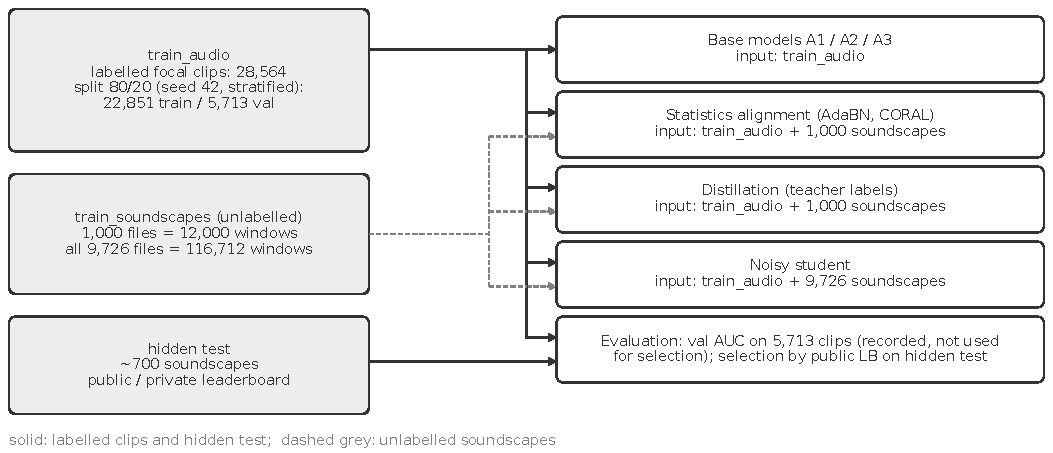
\includegraphics[width=0.85\textwidth]{figures/fig_f2_data_flow.pdf}
\caption{Data flow. Focal clips (\texttt{train\_audio}, 28,564) are split 22,851/5,713 for training and validation. Unlabeled \texttt{train\_soundscapes} are used in two amounts: 1,000 files (12,000 windows) for adaptation and distillation, and all 9,726 files (116,712 windows) for the noisy-student round. The hidden test soundscapes are scored on a public and a private part. No soundscape label is used anywhere. Counts are from our run logs.}
\label{fig:data}
\end{figure*}

\section{Methods}
Figure~\ref{fig:arch} gives the final system. Every model outputs 206 sigmoid probabilities per window.

\begin{figure*}[t]
\centering
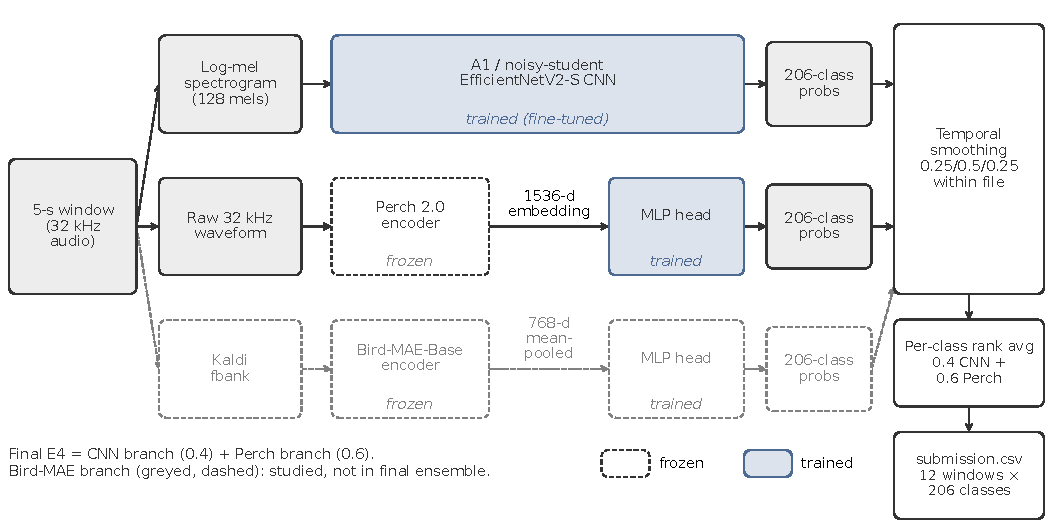
\includegraphics[width=\textwidth]{figures/fig_f1_architecture.pdf}
\caption{System architecture. A five-second window feeds a log-mel CNN, or frozen Perch 2.0 (1536-d embedding) followed by an MLP head, or frozen Bird-MAE-Base followed by an MLP head. Each branch outputs 206-class probabilities, which are smoothed over neighboring windows and combined by a per-class rank average. Frozen and trained components are marked in the figure. The Bird-MAE branch is not in the final ensemble.}
\label{fig:arch}
\end{figure*}

\subsection{Baseline and pretrained models}
\paragraph{v2.}
EfficientNet-B0 with ImageNet weights on a log-mel input (128 bands, $n_\mathrm{fft}=2048$, hop 512, 50--14,000 Hz at 32 kHz; decibels relative to the window maximum, 80 dB range, scaled to $[0,1]$). Training uses random five-second crops of cached spectrograms, soundscape noise (probability 0.5, $-20$ to $-3$ dB), mixup (probability 0.5, Beta(0.4, 0.4)), secondary labels at 0.5, binary cross-entropy, AdamW at $10^{-3}$ (one-cycle), batch 64, 15 epochs.

\paragraph{A1: supervised bird CNN.}
A1 replaces the B0 with the \texttt{tf\_efficientnetv2\_s\_in21k} backbone pretrained on bird audio by the second-place team \citep{sydorskyi2025tackling}, fine-tuned end to end with v2's recipe on the same cached spectrograms. This is a backbone change, not a weights-only swap, because the released dataset has no B0. Weights loaded for 774 of 780 keys; \texttt{conv\_head} and \texttt{bn2} start random. The normalization only partly matches the pretraining front end (80 dB floor, fmax 14 kHz against 16 kHz, fmin 50 Hz against 20 Hz).

\paragraph{A2: supervised multi-taxa, frozen.}
A2 freezes Perch 2.0 \citep{vanmerrienboer2025perch}, run through a community ONNX conversion. It embeds up to 30 s of each focal clip (106,157 windows). An MLP head (512 hidden units, dropout 0.3) is trained on the cached, standardized embeddings with targets 1.0 (primary) and 0.5 (secondary), each window weighted by one over its clip's window count. Perch's own class logits are not used.

\paragraph{A3: self-supervised, frozen.}
A3 freezes Bird-MAE-Base \citep{rauch2025can}, a ViT-B/16 giving 768-d mean-pooled patch tokens, at a pinned commit. Its own Kaldi-style filterbank (128 bins, 512 frames) replaces the log-mel front end, so features come from audio, one window at a time. The MLP head (512 hidden units, dropout 0.2) is trained like A2's.

\subsection{Label-free adaptation}
All adaptation uses unlabeled \texttt{train\_soundscapes} audio (Figure~\ref{fig:methods}).

\begin{figure*}[t]
\centering
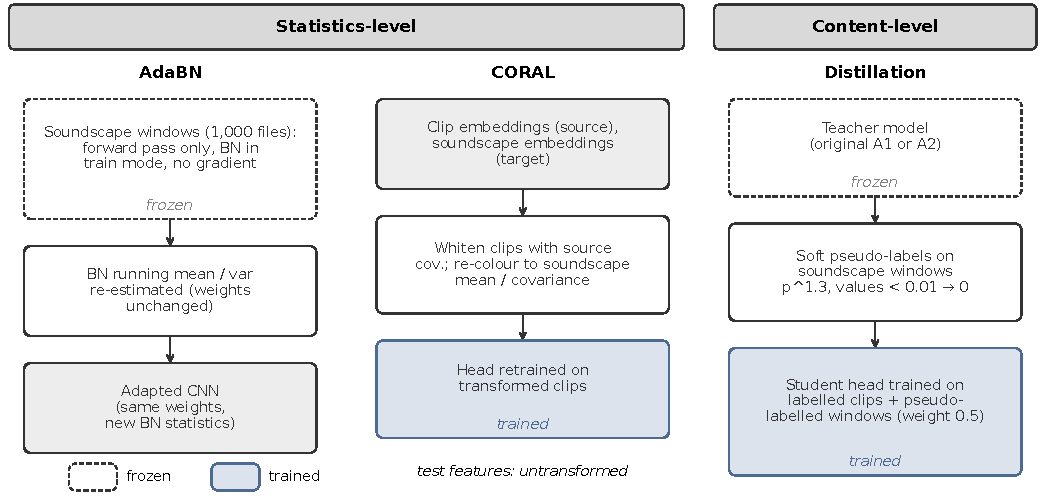
\includegraphics[width=\textwidth]{figures/fig_f3_adaptation_methods.pdf}
\caption{Adaptation methods. Statistics-level: AdaBN re-estimates batch-norm means and variances of a CNN on soundscape windows, and CORAL or mean/std matching maps focal-clip embeddings toward soundscape statistics before the head is trained. Content-level: a teacher labels soundscape windows and a student head or CNN is trained on those pseudo-labels together with the real labels.}
\label{fig:methods}
\end{figure*}

\paragraph{Statistics-level.}
\emph{AdaBN} resets all batch-norm running statistics (110 modules in A1, 49 in v2) and re-estimates them on 12,000 soundscape windows (187 batches of 64) with no weight update \citep{li2018adaptive}. \emph{Mean/std matching} maps a focal embedding $x$ to $(x-\mu_s)/\sigma_s\cdot\sigma_t+\mu_t$ per dimension, with $s$ the focal and $t$ the soundscape statistics. \emph{Standardized CORAL} standardizes each dimension, whitens with the focal correlation matrix, re-colors with the soundscape correlation matrix, then rescales and shifts \citep{sun2016return}, with a ridge of 1.0. The head is trained on mapped focal embeddings and applied to raw soundscape embeddings. Statistics come from 12,000 windows of 1,000 files.

\paragraph{Content-level: head distillation.}
A teacher labels the 12,000 soundscape windows. Teacher probabilities $p$ become soft labels $p^{1.3}$, with values below 0.01 set to 0. The student MLP head trains on the real focal labels plus these windows at loss weight 0.5. Two pairs were run: Perch head (A2) to Bird-MAE head (A3d), and the A1 CNN to the Perch head (A2d).

\paragraph{Content-level: noisy student.}
Figure~\ref{fig:ns} shows round 1. Teachers label all 116,712 windows of the 9,726 files. The MAIN teacher is the mean of A1 and A2 probabilities, the ABLATION teacher is A2d alone; both are sharpened with $p^{1.3}$ and a 0.01 floor. The student is a fresh V2-S from the same bird-pretrained checkpoint, not initialized from A1. Each epoch uses the 22,851 focal clips plus 30,000 soundscape windows from 2,500 files (loss weight 1.0 and 0.5), mixup over the combined batch, stochastic depth 0.15, soft-target binary cross-entropy, and v2's optimizer, schedule and 15 epochs. Soundscape mels are computed on the GPU and were checked against the librosa path used for A1 (maximum input difference $1.3\times10^{-4}$, no changed argmax).

\begin{figure*}[t]
\centering
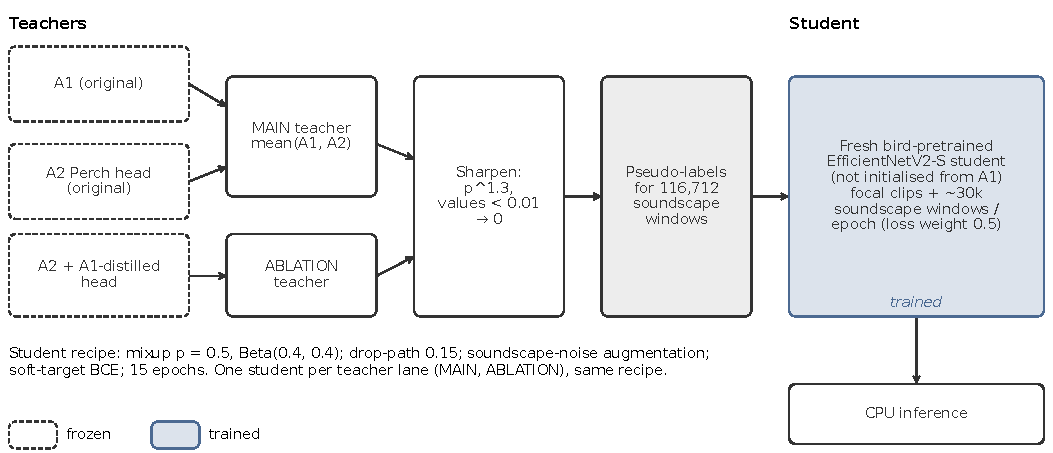
\includegraphics[width=\textwidth]{figures/fig_f4_noisy_student.pdf}
\caption{Noisy student, round 1. Teachers A1 and A2 (MAIN, mean of the two) or A2d (ABLATION) label all 116,712 soundscape windows. Labels are sharpened ($p^{1.3}$, values below 0.01 set to 0) and a freshly initialized bird-pretrained V2-S student is trained on focal clips plus pseudo-labeled windows. MAIN labels have 2.50\% non-zero entries and ABLATION labels 0.74\%, so the two arms differ in teacher and in label density.}
\label{fig:ns}
\end{figure*}

\subsection{Ensemble}
Each model's window probabilities are smoothed within a file,
\begin{equation}
p'_t = 0.25\,p_{t-1} + 0.5\,p_t + 0.25\,p_{t+1},
\end{equation}
with renormalized weights at the first and last window. Scores are combined by a per-class weighted rank average over all test rows,
\begin{equation}
s_{r,c} = \sum_m w_m\,\mathrm{rank}_c\!\big(p^{(m)}_{r,c}\big)\Big/\sum_m w_m ,
\end{equation}
with ranks scaled to $[0,1]$. ROC-AUC depends only on order within a class, so the rank average removes the different probability scales of the models.

\subsection{Bias initialization}
Default initialization starts every class near probability 0.5, although most classes are absent from most windows. The alternative sets the output bias to $b_c=\log\frac{p_c}{1-p_c}$, with $p_c$ the weighted fraction of training windows labeled with class $c$ \citep{lin2017focal}. On Bird-MAE features the mean log-prior is $-6.20$ (range $-9.34$ to $-3.10$).

\section{Experimental Setup}
\paragraph{Protocol.}
All runs use v2's split and recipe. Training and embedding ran on Kaggle T4 GPUs (about 5.6 GPU hours of a 30 hour weekly quota); inference ran on Kaggle CPU with internet off. Each variant was submitted once, and we report public and private scores together.

\paragraph{What was decided before the scores.}
Validation AUC is recorded but never used for selection. Variants and selection rules were written down before the scores they govern, except where noted. The CORAL phase fixed standardized CORAL as MAIN and mean/std as SECONDARY before any score of that phase. The distillation variants (A3d MAIN, A3d with CORAL SECONDARY) and the rule for submitting the secondary one were written after the distillation notebooks were built and pushed, but before any distillation result was seen; the four CORAL scores were also still pending. The A2d specification was fixed before its result. Noisy-student MAIN and ABLATION were pre-registered with a teacher rule, but the final teacher choice (MAIN equals mean of A1 and A2; ABLATION equals A2d) was made on 10 November, \emph{after} the A2d score was known. It is therefore a post-score choice. The ensemble variants E1 to E4, weights and smoothing kernel were fixed before any ensemble score, and the final pick followed the stated rule: highest public score. One control was requested \emph{after} a score: the unadapted A1 scored through the fast inference notebook, requested after the AdaBN score to check the inference path.

\paragraph{Noise level and selection.}
Following the baseline author, we treat public differences below 0.01 as noise and select by public score, because local validation did not predict it. Head seed repeats (seeds 42 to 44, split fixed) give a validation standard deviation of at most 0.0008. Leaderboard noise itself was not measured.

\paragraph{CPU gate.}
Each submission needed a dry run projecting at most 75 minutes for 700 files (hard limit 90). \emph{Measured} times come from a 700-file run on \texttt{train\_soundscapes}; \emph{projected} times scale up a 20-file dry run. Kaggle's tool does not report the scored runtime.

\section{Results}
\subsection{Three pretraining paradigms}
\begin{table}[t]
\centering
\small
\begin{tabular}{lccccc}
\toprule
Model & Val & Pub. & Priv. & Gap p/q & CPU min \\
\midrule
v2 (B0) & 0.9766 & 0.763 & 0.789 & .214/.188 & 11.1 m \\
A1 V2-S & 0.9832 & 0.828 & 0.816 & .155/.167 & 8.0 m \\
A2 Perch & 0.9916 & \textbf{0.848} & \textbf{0.852} & .144/.139 & 25.0 p \\
A3 Bird-MAE & 0.9749 & 0.776 & 0.780 & .199/.195 & 61.6 p \\
\bottomrule
\end{tabular}
\caption{Base models, one submission each. Val is first-5s validation AUC; Gap p/q is validation minus public/private. Exact scores: A1 0.82822/0.81642, A2 0.84774/0.85226, A3 0.77640/0.78016. CPU minutes for 700 files: m measured, p projected. v2 time is its profile run; A1 time is through the fast pipeline (the submitted A1 notebook projects to about 37). v2's validation AUC is from the clean-validation line of the v2 AdaBN run.}
\label{tab:base}
\end{table}

Perch 2.0 is best (public +0.085 over v2, private +0.063), A1 second (+0.065, +0.027) (Table~\ref{tab:base}, Figure~\ref{fig:lb}). A3 is +0.013 public and $-0.009$ private, which we do not read as an improvement; it clears the 0.776 grading cut-off by 0.0004, inside the noise. Perch 2.0 was released after the competition closed.

\begin{figure*}[t]
\centering
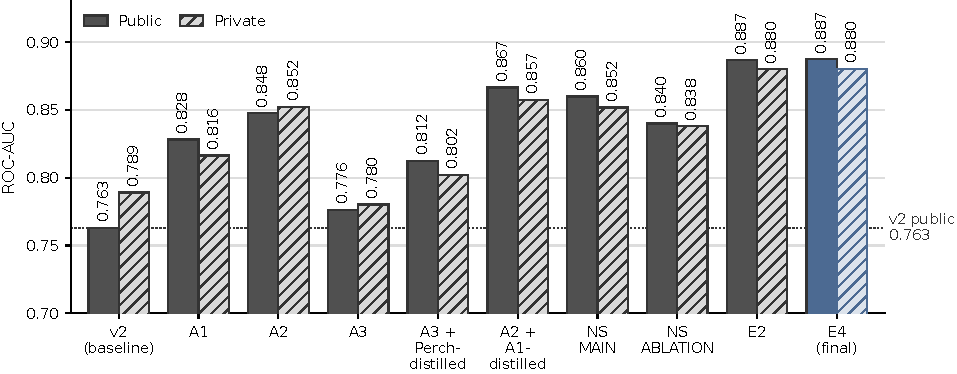
\includegraphics[width=\textwidth]{figures/fig_lb_progression.pdf}
\caption{Public and private leaderboard AUC of ten systems in the order they were built: v2, A1, A2, A3, A3 with Perch distillation, A2 with A1 distillation, noisy-student MAIN and ABLATION, and ensembles E2 and E4. Each value is one late submission, taken from Tables~\ref{tab:base} to~\ref{tab:ens}.}
\label{fig:lb}
\end{figure*}

\subsection{Adaptation study}
Table~\ref{tab:adapt} lists every adaptation submission against its unadapted parent (A1 for the noisy students).

\begin{table*}[t]
\centering
\small
\begin{tabular}{llllrrcc}
\toprule
Model & Method & Level & Pub. & $\Delta$ pub. & $\Delta$ priv. & Gap pub. & Gap priv. \\
\midrule
v2 & AdaBN & statistics & 0.73889 & $-0.0241$ & $-0.0252$ & .214 $\to$ .202 & .188 $\to$ .177 \\
A1 & AdaBN & statistics & 0.77210 & $-0.0561$ & $-0.0507$ & .155 $\to$ .199 & .167 $\to$ .206 \\
A2 & CORAL (main) & statistics & 0.68790 & $-0.1598$ & $-0.1437$ & .144 $\to$ .302 & .139 $\to$ .282 \\
A2 & mean/std & statistics & 0.68728 & $-0.1605$ & $-0.1459$ & .144 $\to$ .304 & .139 $\to$ .285 \\
A3 & CORAL (main) & statistics & 0.64281 & $-0.1336$ & $-0.1333$ & .199 $\to$ .330 & .195 $\to$ .326 \\
A3 & mean/std & statistics & 0.66971 & $-0.1067$ & $-0.0998$ & .199 $\to$ .305 & .195 $\to$ .295 \\
A3 & Perch-distilled + CORAL & both & 0.69343 & $-0.0830$ & $-0.0916$ & .199 $\to$ .279 & .195 $\to$ .284 \\
\midrule
A3 & Perch-distilled (A3d) & content & 0.81238 & $+0.0360$ & $+0.0219$ & .199 $\to$ .163 & .195 $\to$ .173 \\
A2 & A1-distilled (A2d) & content & 0.86651 & $+0.0188$ & $+0.0051$ & .144 $\to$ .125 & .139 $\to$ .134 \\
A1 & noisy student, MAIN & content & 0.85985 & $+0.0316$ & $+0.0354$ & .155 $\to$ .127 & .167 $\to$ .135 \\
A1 & noisy student, ABLATION & content & 0.84003 & $+0.0118$ & $+0.0215$ & .155 $\to$ .145 & .167 $\to$ .147 \\
\bottomrule
\end{tabular}
\caption{Adaptation against the unadapted parent. $\Delta$ is the change in public or private score; Gap is validation minus leaderboard AUC, parent $\to$ adapted. The ``both'' row combines CORAL on the training features with distillation. Public differences below 0.01 are treated as noise; the A2d private change ($+0.0051$) is within that range. A1 AdaBN was checked with a control: the unadapted A1 through the same fast notebook scored 0.82822/0.81642, identical to the original, so the drop is due to AdaBN. The v2 gap narrows only because validation AUC fell (0.9766 to 0.9405) more than the leaderboard score.}
\label{tab:adapt}
\end{table*}

Statistics-level alignment lowered the public score in every case, by $0.024$ to $0.160$, and the private score by similar amounts, although focal validation AUC barely moved for the frozen encoders (Perch 0.9916 to 0.9901). The loss was largest for frozen embeddings. AdaBN hurt the ImageNet model less than the bird-pretrained one ($-0.024$ against $-0.056$ public); with one model of each kind, we do not attribute this to the pretraining.

Content-level adaptation raised the public score in all four cases, by $+0.012$ to $+0.036$, and narrowed the gap each time (Figure~\ref{fig:delta}). All four public gains exceed the 0.01 noise level, the ABLATION student only narrowly ($+0.0118$). The private gain of A2d ($+0.0051$) is within noise. Distillation combined with CORAL recovered $+0.051$ over A3 with CORAL alone but ended at $-0.083$ public, far below the unadapted A3.

\begin{figure}[t]
\centering
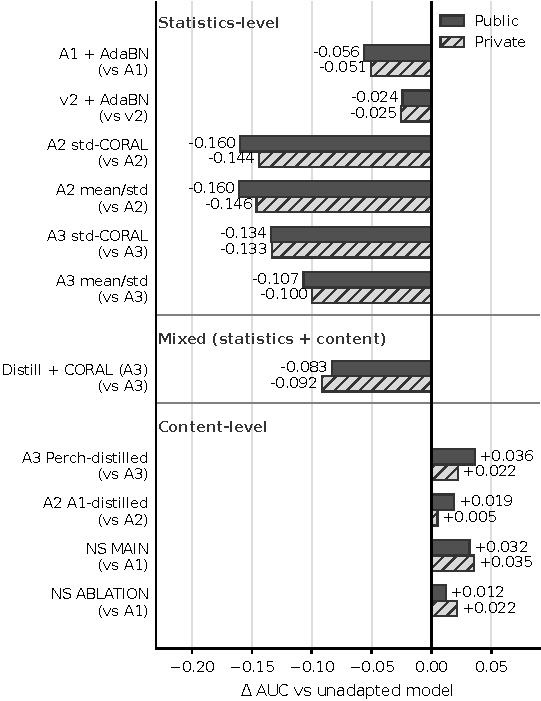
\includegraphics[width=\columnwidth]{figures/fig_adaptation_delta.pdf}
\caption{Change in public and private leaderboard AUC against the unadapted parent, for every submission of Table~\ref{tab:adapt}, grouped as statistics-level, mixed (distillation with CORAL-mapped training features) and content-level. Dark bars are public, hatched bars private; each pair is one late submission. The horizontal axis is the change in AUC; zero means no change. Noisy-student rows are compared with A1.}
\label{fig:delta}
\end{figure}

\subsection{Distillation and noisy student}
\begin{table}[t]
\centering
\small
\begin{tabular}{llccc}
\toprule
Student & Teacher & Non-zero & Pub. & Priv. \\
\midrule
A3d head & A2 (Perch) & 1.9\% & 0.81238 & 0.80208 \\
A2d head & A1 CNN & 3.7\% & 0.86651 & 0.85737 \\
\bottomrule
\end{tabular}
\caption{Head distillation on 12,000 soundscape windows (1,000 files). Non-zero is the share of non-zero label entries after sharpening. Students are compared with A3 (0.77640/0.78016) and A2 (0.84774/0.85226).}
\label{tab:dist}
\end{table}

In Table~\ref{tab:dist}, A3d learned from the stronger Perch teacher and gained $+0.036$ public. A2d learned from the \emph{weaker} A1 teacher (0.828 public against A2's 0.848) and still improved, by $+0.0188$ public and $+0.0051$ private (within noise). This is consistent with the two models making different errors: the per-class Spearman correlation between A1 and A2 probabilities on soundscape windows is only 0.31 (mean over classes, 20,000 windows). We did not test that explanation.

\begin{table}[t]
\centering
\small
\begin{tabular}{lcc}
\toprule
 & MAIN & ABLATION \\
\midrule
Teacher & mean(A1, A2) & A2d \\
Non-zero labels & 2.50\% & 0.74\% \\
Windows with label $\ge0.5$ & 11,430 & 7,952 \\
Best val AUC & 0.9865 & 0.9854 \\
Public & \textbf{0.85985} & 0.84003 \\
Private & \textbf{0.85185} & 0.83794 \\
$\Delta$ vs A1 (pub./priv.) & +.0316/+.0354 & +.0118/+.0215 \\
Gap val$-$pub. & 0.127 & 0.145 \\
CPU min & 9.9 m & 10.0 m \\
\bottomrule
\end{tabular}
\caption{Noisy student round 1. Both arms use the same student and recipe. Val AUC is first-5s and was not used for selection. A1 reference: 0.82822/0.81642, val 0.9832, gap 0.155. m: measured on 700 files.}
\label{tab:ns}
\end{table}

In Table~\ref{tab:ns}, MAIN beats ABLATION by $+0.0198$ public and $+0.0139$ private, above the noise level, and gains $+0.0316$ and $+0.0354$ over its teacher A1 at 9.9 CPU minutes against 8.0. Neither student beats A2d (0.86651/0.85737). The arms differ in teacher \emph{and} label density (2.50\% against 0.74\% non-zero entries), so the difference cannot be assigned to the teacher alone; we ran no density-matched control. Validation curves differ by at most 0.002 at the end (Figure~\ref{fig:curves}), so validation could not choose between the arms.

\begin{figure}[t]
\centering
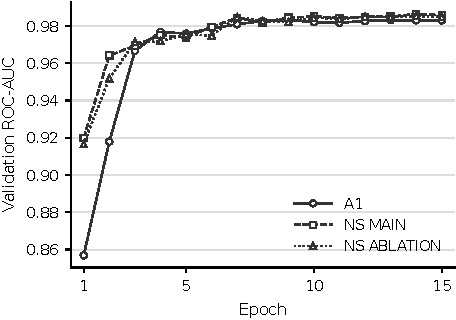
\includegraphics[width=\columnwidth]{figures/fig_training_curves.pdf}
\caption{First-5s validation AUC per epoch for A1, noisy-student MAIN and noisy-student ABLATION (clean focal validation, 15 epochs each, one seed). Best epochs are 9 for A1 (0.9832) and 14 for both students (0.9865 and 0.9854). The students train on 22,851 focal clips plus pseudo-labeled soundscape windows, A1 on clips only.}
\label{fig:curves}
\end{figure}

\subsection{Ensemble}
\begin{table}[t]
\centering
\small
\begin{tabular}{llccc}
\toprule
 & Weights; smoothing & Pub. & Priv. & CPU min \\
\midrule
E1 & .5/.5; no & 0.88352 & 0.87203 & 28.3 m \\
E2 & .5/.5; yes & 0.88662 & 0.88008 & 30.4 m \\
E3 & 1/3 each (+ABL.); yes & 0.88058 & 0.87522 & 39.9 m \\
E4 & .4/.6; yes & \textbf{0.88749} & \textbf{0.88029} & 32.3 m \\
\bottomrule
\end{tabular}
\caption{Rank-average ensembles of the MAIN student and A2d (weights in that order; E3 adds the ABLATION student). Best single model A2d: 0.86651/0.85737. Smoothing kernel 0.25/0.5/0.25. E4 is the pre-registered pick. m: measured on 700 files.}
\label{tab:ens}
\end{table}

In Table~\ref{tab:ens}, E1 beats the best single model A2d by $+0.0170$ public and $+0.0147$ private, so the CNN and the Perch head are complementary. Smoothing adds $+0.0031$ public (noise) and $+0.0081$ private. E3 is below E2 on both splits: a second CNN moved weight away from Perch. E4 and E2 differ by $+0.0009$ and $+0.0002$ and are equivalent. E4 reached 0.88749 public and 0.88029 private, $+0.124$ and $+0.091$ over v2.

\subsection{Seed repeats}
\begin{table}[t]
\centering
\small
\begin{tabular}{lc}
\toprule
Head & Val AUC, mean $\pm$ std \\
\midrule
A2 original & 0.99163 $\pm$ 0.00029 \\
A3 original & 0.97451 $\pm$ 0.00076 \\
A2d & 0.99133 $\pm$ 0.00047 \\
A3d & 0.97506 $\pm$ 0.00012 \\
\bottomrule
\end{tabular}
\caption{Seeds 42 to 44, first-5s validation AUC, sample standard deviation over three CPU runs. Only the heads were repeated; the split is fixed. The CNNs were trained once.}
\label{tab:seed}
\end{table}

Table~\ref{tab:seed} shows head-level seed noise of at most 0.0008. The validation differences between the CORAL-family heads and their controls (at most about 0.002) are a few such standard deviations, whereas the leaderboard changes of the same variants are 0.08 to 0.16.

\subsection{Bird-MAE: a linear probe that looked poor}
A linear probe on standardized mean-pooled Bird-MAE features reached 0.7498 first-5s validation AUC (0.7495 on the first run). Its first-epoch loss was 0.6941, close to $\ln 2$, and it plateaued at 0.277. Raising the learning rate from $10^{-3}$ to $3\times10^{-3}$ and $10^{-2}$ raised the AUC to 0.8513 and 0.9370. Initializing the output bias to the class log-prior, with nothing else changed, gave 0.9626 and a first-epoch loss of 0.0285. An analytical estimate suggests the default bias could move by only about 1.3 over the whole schedule, short of the roughly $-6$ needed; we did not measure the bias trajectory. The same trick did not help the MLP head (0.9707 against 0.9749), and the default-bias MLP was submitted as A3. The Perch logistic regression showed the same plateau (loss 0.278, AUC 0.9071) and was not rerun, so we only presume the same defect; the A2 MLP is unaffected.

\section{Discussion}
\subsection{The transfer gap}
\begin{figure}[t]
\centering
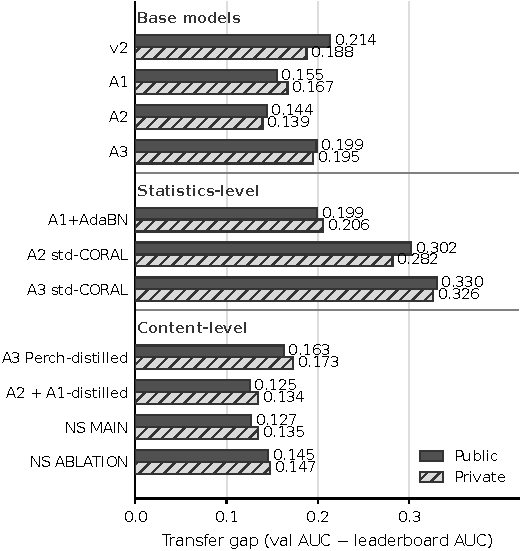
\includegraphics[width=\columnwidth]{figures/fig_transfer_gap.pdf}
\caption{Transfer gap (first-5s validation AUC minus public or private leaderboard AUC) for the base models, three statistics-level variants (A1 AdaBN and the two standardized-CORAL heads) and the four content-level models of Table~\ref{tab:adapt}. Dark bars are public, hatched bars private. Single seed and split. Validation is macro AUC over held-out focal clips (191 classes with positives) and the leaderboard is macro AUC on soundscapes, so the gap mixes domain shift with class coverage and is descriptive only.}
\label{fig:gap}
\end{figure}

All base models have a large gap (Figure~\ref{fig:gap}): A2 0.144, A1 0.155, A3 0.199, v2 0.214 on the public part. Clean validation ordered A1, A2 and A3 as the leaderboard did but compressed the spread: validation spans 0.017, public scores 0.071. A2's validation AUC may be inflated, because Perch was trained on Xeno-canto and iNaturalist, which \texttt{train\_audio} also draws from; we did not check the overlap. Content-level adaptation narrowed the gap by 0.010 to 0.036 public; statistics-level adaptation widened it in six of seven cases.

\subsection{Why statistics alignment failed}
The drops were large while validation barely changed, so a pipeline bug was the first suspect. A diagnostic notebook found none: with the original A2 head, the CORAL inference path and the original notebook differ by at most $3.0\times10^{-8}$ on 240 rows (threshold $10^{-5}$), and the saved head means match the soundscape means as intended.

We had pre-registered one explanation, H1: adapted heads give much higher probabilities on background windows, because the mean shift maps typical soundscape onto typical call clips. On 12,000 soundscape windows H1 is not supported. Mean probability rose only for Perch mean/std (0.0035 to 0.0044) and fell elsewhere, and the share of windows with a maximum above 0.5 fell in every case. What changed instead was the ranking within each class: the mean per-class Spearman correlation with the original head is 0.29 to 0.37 for Perch and 0.57 to 0.72 for Bird-MAE. ROC-AUC is sensitive to exactly this. Among the A3 variants the lower-correlation one (CORAL, 0.57) also scored 0.03 lower than mean/std (0.72), while for Perch both correlate poorly and score alike. This is an association across four points, not proof.

Two further explanations are hypotheses and untested. First, soundscape statistics are dominated by windows with no target species, so aligning to them may move a call-bearing focal clip toward background. Second, the CORAL ridge of 1.0 is large against per-dimension variances near 0.01 to 0.02, so the raw variant is nearly a mean shift; we trained but did not submit it.

\subsection{Why pseudo-labels helped}
Content-level adaptation changes what the model sees rather than how its features are scaled. Our hypothesis is that pseudo-labeled soundscape windows teach the student what real background looks like, including that most windows hold no target species, while soft labels carry the teacher's knowledge. Three observations bear on it. A3d, whose head had seen only clean clips, gained after seeing soundscape windows, which is consistent with clean-only training being part of the gap but is confounded by the teacher's labels. A2d learned from a weaker teacher of another family and still improved, in line with the motivation for cross-lineage teachers in \citet{farazi2026crossmutated}; our two head-distillation runs are too few to test that idea. CORAL on top of distillation destroyed most of the gain, so the damage from the mapping survives pseudo-labels. The MAIN-ABLATION difference could come from teacher, label density, or both.

\subsection{Why Bird-MAE transferred worst}
A3 had the largest gap. We offer three hypotheses, none tested directly.
\begin{description}
\item[P1: mean pooling dilutes short calls.] A short call occupies few of the 256 patch tokens. Bird-MAE's paper reports that prototypical probes on the full patch map beat linear probes by up to 37 points mAP \citep{rauch2025can}, on a different metric and datasets. We did not run one. Perch also gives one vector per window, which weakens the argument.
\item[P2: the head saw only clean clips.] A3's head and A2's head were both trained on clean-clip embeddings with no augmentation, and A2 transferred best, so P2 cannot explain the A2--A3 difference alone. The gain of A3d is consistent with P2 but not a test of it.
\item[P3: pretraining objective and data.] Perch is supervised on multi-taxa recordings; Bird-MAE is self-supervised on bird recordings. A supervised objective may separate species better under noise, and a bird-only set may serve the 60 non-bird classes less well. The models also differ in size, data volume and release date. We have no per-taxon leaderboard score to test this.
\end{description}
Even after the bias repair, the Bird-MAE MLP head transferred worst. A first-epoch loss near $\ln 2$ and a high plateau were the warning that the default probe (0.21 AUC below the log-prior probe) measured initialization, not features.

\subsection{Speed}
Profiling v2 on 700 files with its own pool took 11.1 minutes (10.4 for the pipeline). Mel computation was the largest part: 1,078 of 1,590 summed seconds across decode, mel and model. The fast pipeline uses four file-level workers with one thread each, one mel call on the 12 windows of a file, and one model batch per file. It cut v2 to 5.5 minutes (pipeline 4.0) and ran A1 in 8.0; summed mel seconds fell from 1,078 to 314. We did not isolate which change mattered, and the model-stage numbers of the two runs are not comparable (main-process wall time on four threads against a sum over four single-thread workers). The baseline author's figure of about 25 minutes was not reproduced. ONNX Runtime and OpenVINO runs for the CNNs were not done; an OpenVINO FP16 smoke test ran as float32 with no speedup.

\begin{figure*}[t]
\centering
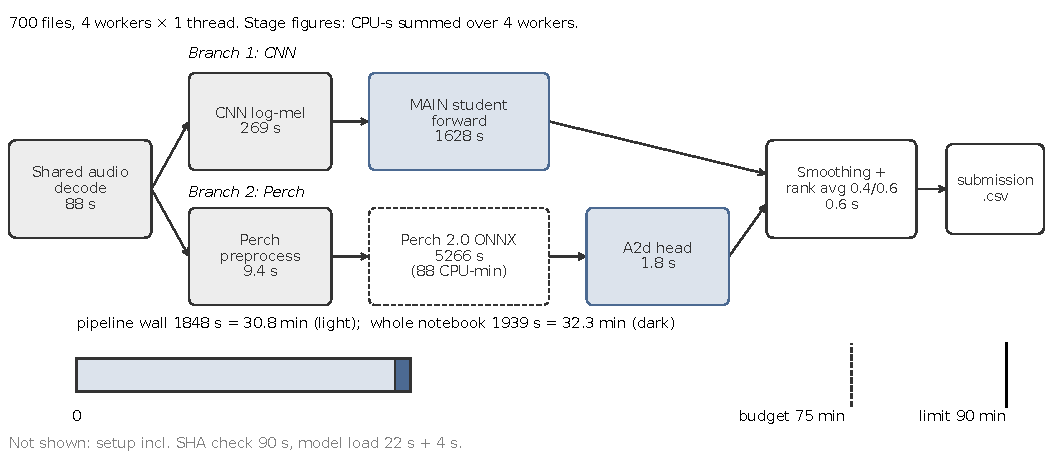
\includegraphics[width=\textwidth]{figures/fig_f5_inference_pipeline.pdf}
\caption{Final E4 CPU inference pipeline with measured per-stage CPU seconds summed over four workers (decode 87.8, CNN mel 268.7, student CNN 1,628.1, Perch branch 5,265.7). The Perch branch is about 73\% of the summed stage time. The whole notebook took 32.3 minutes on 700 files, against the 75-minute budget and the 90-minute limit. Summed seconds are CPU time and do not add up to wall time.}
\label{fig:pipe}
\end{figure*}

\begin{figure}[t]
\centering
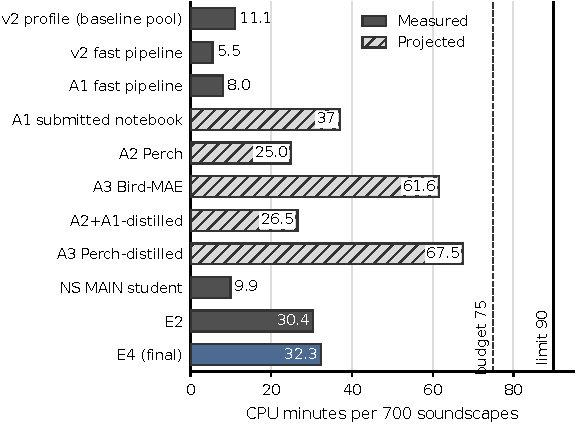
\includegraphics[width=\columnwidth]{figures/fig_timing.pdf}
\caption{CPU minutes for 700 one-minute files for each pipeline, shown as measured (full 700-file run) or projected (scaled from a 20-file dry run), with the 75-minute budget and 90-minute limit. Projected values may be pessimistic because worker start-up is spread over only 20 files.}
\label{fig:timing}
\end{figure}

In the final system (Figure~\ref{fig:pipe}) the Perch encoder dominates the cost, and E4 ran in 32.3 minutes (Figure~\ref{fig:timing}), well under the 75-minute budget. E3 needed 39.9 minutes. Bird-MAE at 61.6 projected minutes would leave little room for a second model.

\subsection{Comparison with published 2025 scores}
The top of the Kaggle final leaderboard was 0.93067 (first) and 0.92893 (second)\footnote{Final leaderboard of BirdCLEF+ 2025, read with the Kaggle command-line tool on 10 November 2026: \url{https://www.kaggle.com/competitions/birdclef-2025/leaderboard}.}. The second-place solution, whose pretrained backbone we use, is described by \citet{sydorskyi2025tackling}. E4's private score of 0.88029 is 0.050 and 0.049 below these. The best model-zoo model of DS@GT scored 0.778 private and 0.810 public \citep{miyaguchi2025distilling}, below E4 on both. These comparisons need care. Our submissions are late and unranked. Perch 2.0 appeared in August 2025, after the competition closed in June, so competitors could not use it. We had a course compute budget, made 19 submissions, and selected on the public score. We claim no rank and do not read the gap to the top as a measure of method quality.

\section{Limitations}
\begin{itemize}
\item \textbf{Single split, limited seeds.} One stratified split (seed 42). Seeds were repeated only for the small heads; the CNN backbones and students were trained once.
\item \textbf{Public and private noise.} We treat public differences below 0.01 as noise, a rule inherited from the baseline author and not measured by repeated submissions. The two parts disagree on some close calls (E1 against E3).
\item \textbf{Adaptation data.} AdaBN and CORAL used 12,000 windows from 1,000 files. Whether more files would change the result was not tested, so the negative result is specific to this setup.
\item \textbf{Ablation confound.} MAIN and ABLATION differ in teacher and label density.
\item \textbf{Post-score choice.} The MAIN teacher was fixed after the A2d score was known. The A1 control was requested after the AdaBN score.
\item \textbf{Perch 2.0 timing.} It was released on 6 August 2025, after BirdCLEF 2025 closed on 5 June 2025, so A2, A2d and the ensemble are not comparable to official ranks. The ONNX file is a community conversion.
\item \textbf{Training-data overlap.} Perch and \texttt{train\_audio} may share recordings (Xeno-canto, iNaturalist), which can inflate A2's validation AUC. We did not check the overlap.
\item \textbf{Bird-MAE licence.} The weights have no declared licence on the model card, code repository or arXiv listing; they stayed in a private dataset.
\item \textbf{No labeled soundscapes.} Domain-shift explanations could not be tested directly, and the transfer gap mixes shift with class coverage.
\item \textbf{Late submissions are unranked.}
\item \textbf{Timing and A1.} Some CPU times are projections. A1 confounds architecture, pretraining and normalization. v2's score is known to three decimals, so deltas carry up to 0.0005 of rounding. The prototypical probe for Bird-MAE was not run.
\end{itemize}

\section{Future Work}
A multi-round noisy student would test whether the gain compounds or saturates. Pseudo-label filtering by confidence or teacher agreement, with a density-matched control, would separate teacher quality from label density. Sound-event-detection heads and longer context would use temporal structure that we only smooth. A labeled soundscape subset would allow per-taxon evaluation and a test of P1 to P3. External in-domain pretraining and a prototypical probe for Bird-MAE are further directions.

\section{Conclusion}
Frozen Perch 2.0 and a supervised bird CNN transferred from focal clips to soundscapes much better than frozen Bird-MAE-Base, yet all three kept a validation-to-leaderboard gap of 0.14 to 0.20. Aligning feature statistics lowered the public score in every submission (by 0.024 to 0.160); training on teacher pseudo-labels raised it every time (by 0.012 to 0.036), even from a weaker teacher. A rank-average ensemble with temporal smoothing reached 0.88749 public and 0.88029 private in 32.3 CPU minutes. The evidence rests on one split, head-only seeds and late submissions with a model that post-dates the competition, so it is a record of what worked, not a ranking.

\section*{AI-use disclosure}
\textbf{[PLACEHOLDER: AI-use disclosure statement, to be completed by the authors if required by the course.]}

\bibliography{references}

\end{document}
